%%% lorem.tex --- 
%% 
%% Filename: lorem.tex
%% Description: 
%% Author: Ola Leifler
%% Maintainer: 
%% Created: Wed Nov 10 09:59:23 2010 (CET)
%% Version: $Id$
%% Version: 
%% Last-Updated: Wed Nov 10 09:59:47 2010 (CET)
%%           By: Ola Leifler
%%     Update #: 2
%% URL: 
%% Keywords: 
%% Compatibility: 
%% 
%%%%%%%%%%%%%%%%%%%%%%%%%%%%%%%%%%%%%%%%%%%%%%%%%%%%%%%%%%%%%%%%%%%%%%
%% 
%%% Commentary: 
%% 
%% 
%% 
%%%%%%%%%%%%%%%%%%%%%%%%%%%%%%%%%%%%%%%%%%%%%%%%%%%%%%%%%%%%%%%%%%%%%%
%% 
%%% Change log:
%% 
%% 
%% RCS $Log$
%%%%%%%%%%%%%%%%%%%%%%%%%%%%%%%%%%%%%%%%%%%%%%%%%%%%%%%%%%%%%%%%%%%%%%
%% 
%%% Code:

\chapter{Results}
\label{cha:results}
This chapter will present the results of choosing and implementing the different techniques explained in the method. Moreover, images on agar plates before and after using the different techniques will be shown. 

\section{Implementation}
Using a dataset of 300 images, \textit{Figure \ref{fig:result final}} is a general representation of the five most distinctive types of input images of the dataset in terms of rotation, perspective, bacterial growth, lightning, and positioning. Figures throughout the implementation are based on outputs visually and pedagogical enough to prove the method of their respective step. Minor pixel-level variations throughout the dataset could be found, still giving reasonable final results. \\

\noindent The method was implemented using Python 3.8 and the open library OpenCV 4.2. Results were produced on the following hardware: Intel I7-5600 2.59GHz, 8GB DDR3L 1600MHz, and 256GB SSD.



\subsection{Identify and mask the agar plate}
\noindent There is a significant positive relationship with using SCB to intensify the primary colors, brightness, and contrast of images. This result is consistent throughout the image data set, which had varying color and lighting conditions. SCB managed to intensify both brightness and the RGB-colors to give a clearer image and visible agar plate. For pictures with very low brightness (first row in \textit{Figure \ref{fig:result color balance}}), the prior balance of brightness and contrast gave some improvement in the color balance. However, in most cases, there was not any difference, and SCB provided good results on its own (see the second row in \textit{Figure \ref{fig:result color balance}}). \\

\begin{figure}[H]
    \centering
     \includegraphics[width=1.1\linewidth]{figures/PDF/Final_result.pdf}
        \caption{a) Input image. b) The outer contour of the agar plate identified. c) Compartment edges identified. d) Final output.}
    \label{fig:result final}
\end{figure}

\begin{figure}[H]
    \centering
    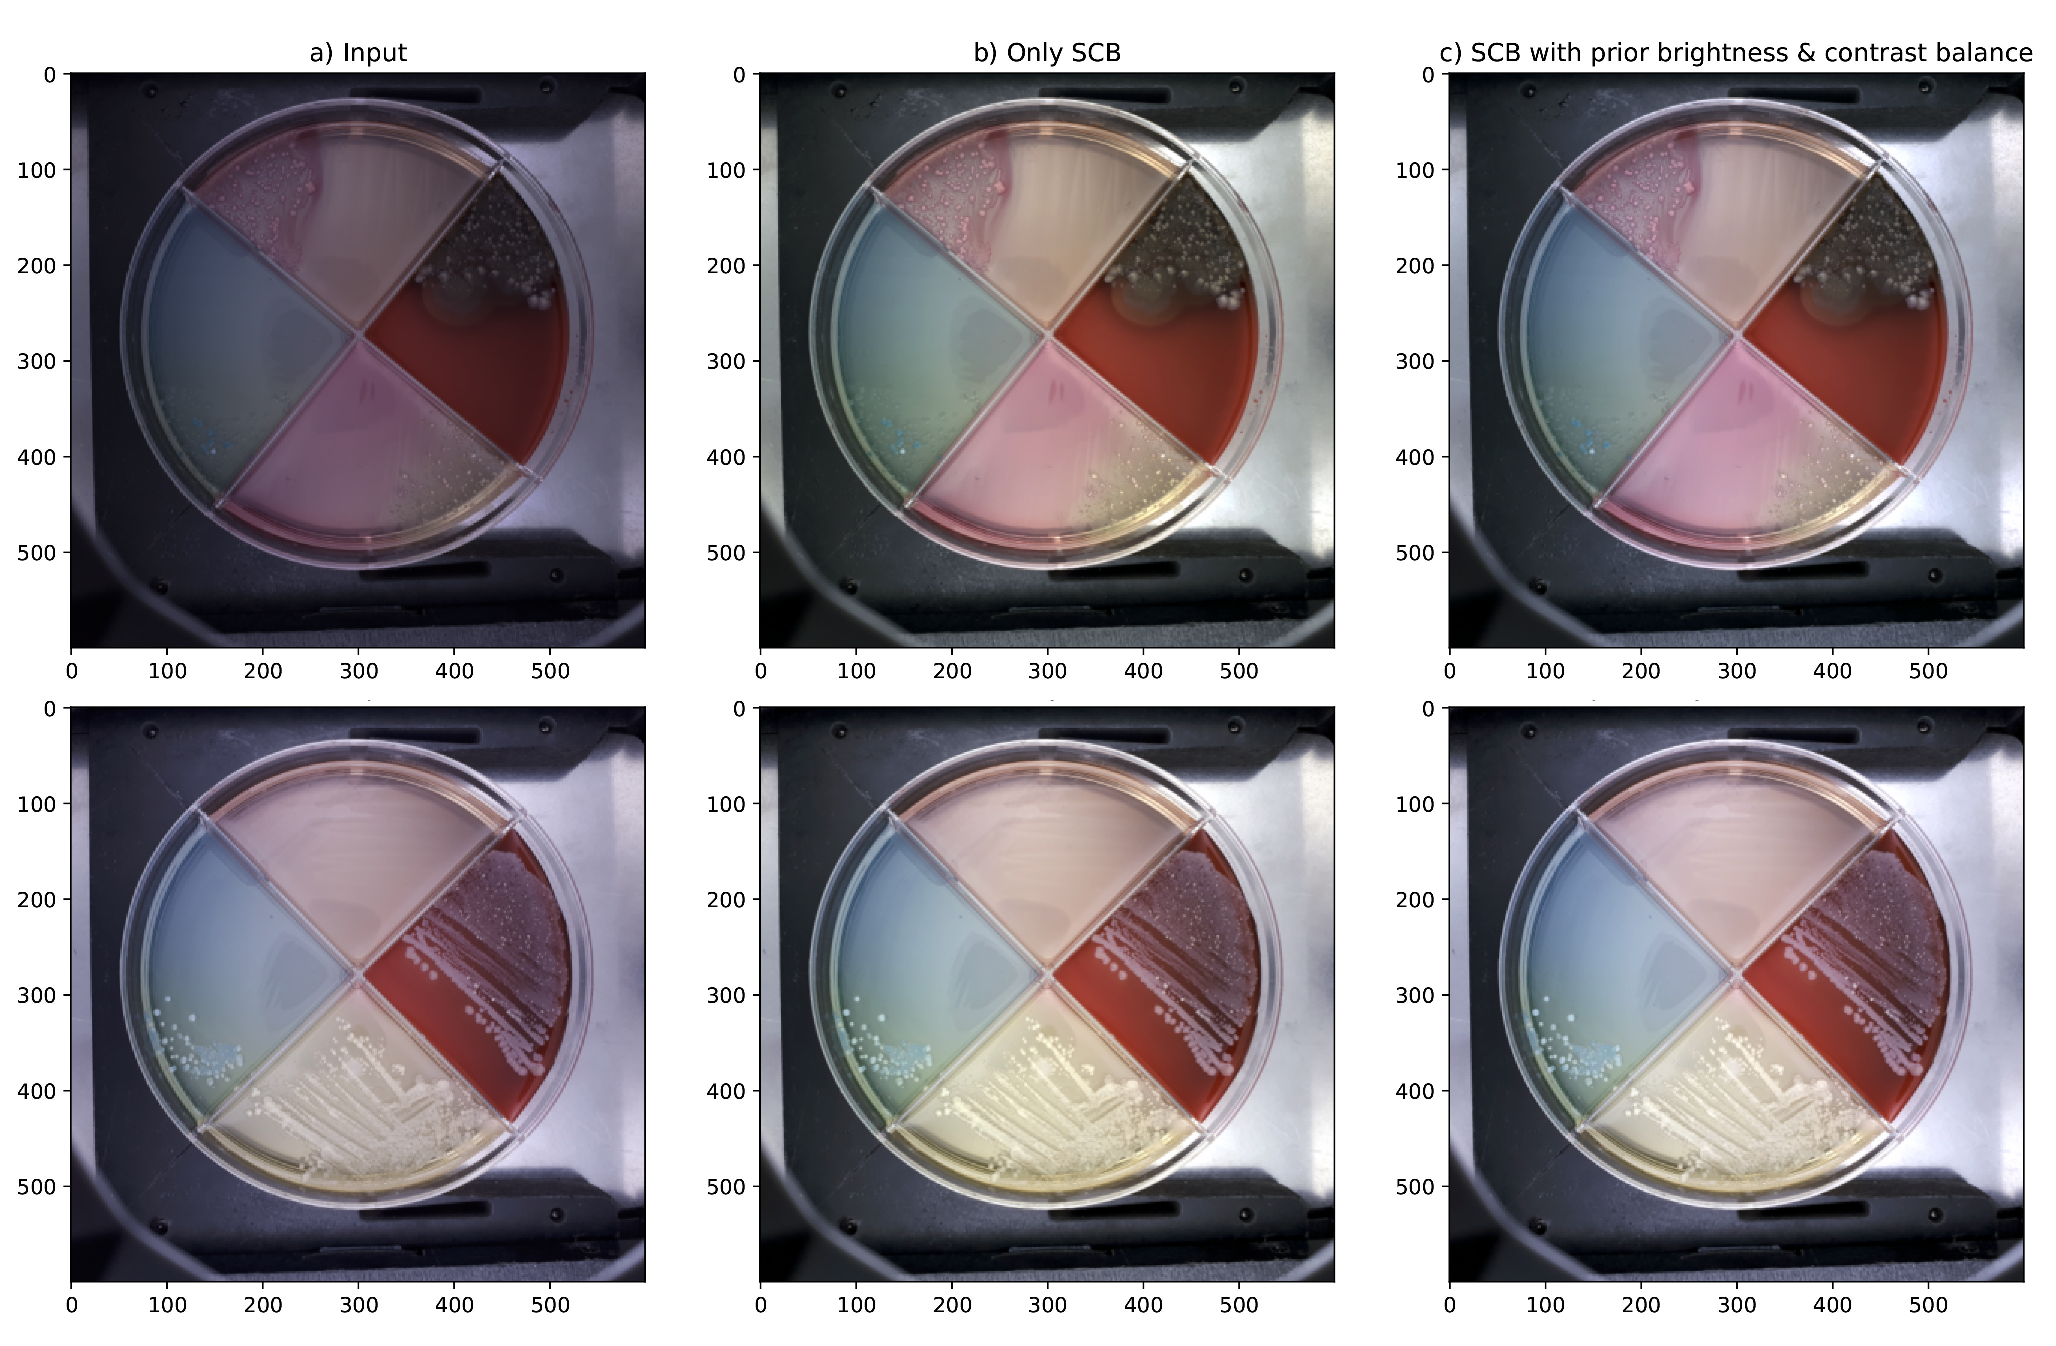
\includegraphics[width=1\linewidth]{figures/PDF/SCB.pdf}\\  
    \caption{a) Input image of an agar plate under dark conditions. b) Image processed with SCB. c) Image processed with SCB with prior brightness and contrast balance  }
    \label{fig:result color balance}
\end{figure}

\noindent As seen in \textit{Figure \ref{fig:result canny}}, Canny proves to be a useful tool for initial edge detection. Adding another iteration of Gaussian blur before Canny, gave a significant improvement in terms of removing image noise such as bacteria clusters and highlighting the actual structure of the agar plate. The result throughout the dataset was mainly dependent on the extent of bacterial growth. Some more extreme cases may have caused the agar plate contour to be connected to features in the background. These deviations were later addressed using RANSAC at the end of this section. For this work, the lower and upper threshold values for Canny were set 0, respectively 255, to keep only the most intense pixels. The Gaussian blur sigma value was set to 0.8. \\

\begin{figure}[H]
    \centering
     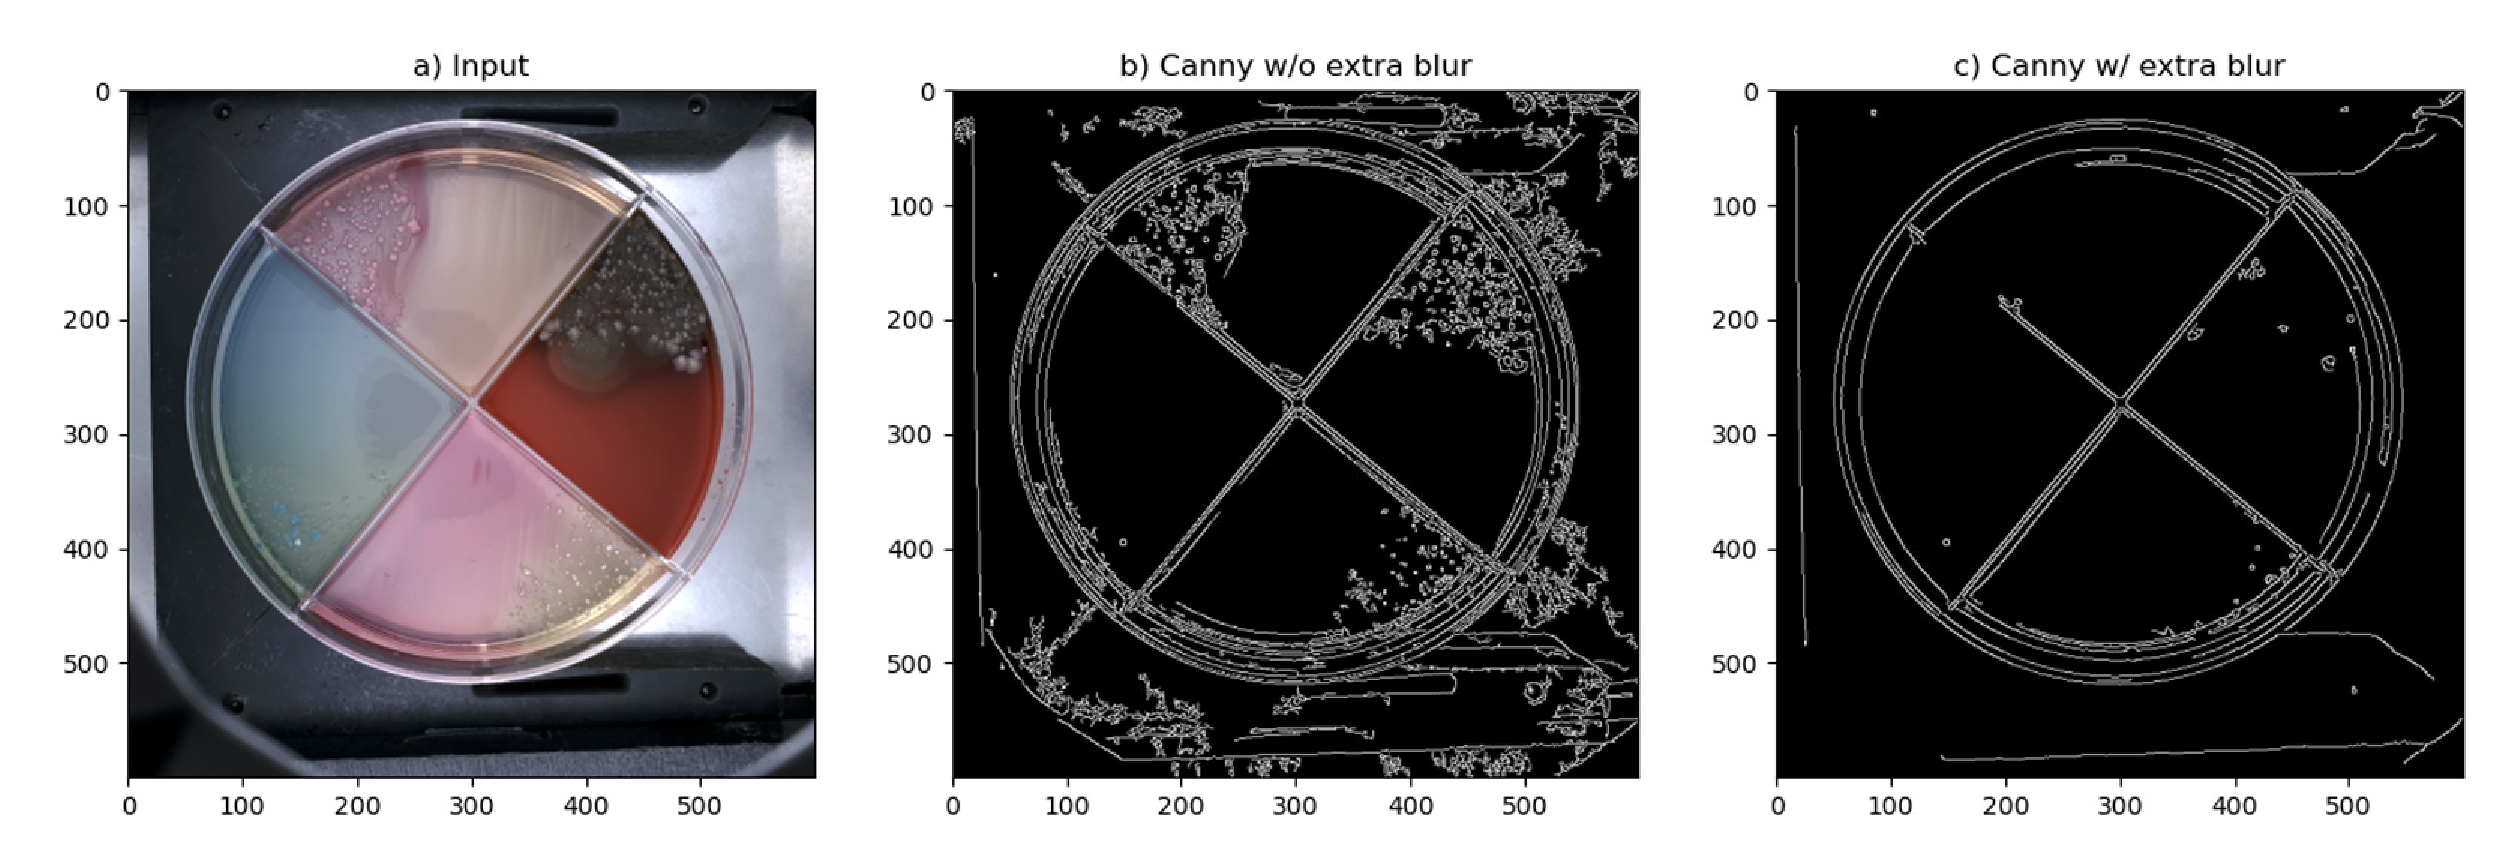
\includegraphics[width=1\linewidth]{figures/PDF/Canny.pdf}\\
    \caption{a) Input image. b) image processed with Canny Edge Detection. c) Image processed with Canny Edge Detection but, with extra Gaussian Blur. }
    \label{fig:result canny}
\end{figure}

\noindent\textit{Figure \ref{fig:result ransac}} shows that RANSAC effectively improves the approximation of the outer contour in deviances occurring during border following. \textit{Figure \ref{fig:result ransac} b)} shows the deviances occurring with Border Following. Closing was made with five iterations of dilation, followed by six iterations of erosion, giving a consistent output for the RANSAC to correct. The sixth iteration of erosion proved useful to remove additional background noise. \\

\noindent Using closing on the Canny output in \textit{Figure \ref{fig:result canny} c)}, the outermost edges could be merged, forming one thick edge, thus providing a more distinctive outer edge, as seen in \textit{Figure \ref{fig:result ransac} a)}.\\

\noindent The found contour was validated with an $ 80\%$ matching rate to their corresponding CHT shape. The matching rate was set a bit lower to cope with the more extreme cases. Images with a matching rate of over $ 85\%$, in this case, proved in general to provide the most accurate results.\\

\noindent RANSAC was set to 100 iterations, which gave accurate results with providing the elliptical contour, as seen in \textit{Figure \ref{fig:result ransac} c)}. However, it was quite time-consuming with a computation time of up to 50 seconds.


\begin{figure}[H]
    \centering
     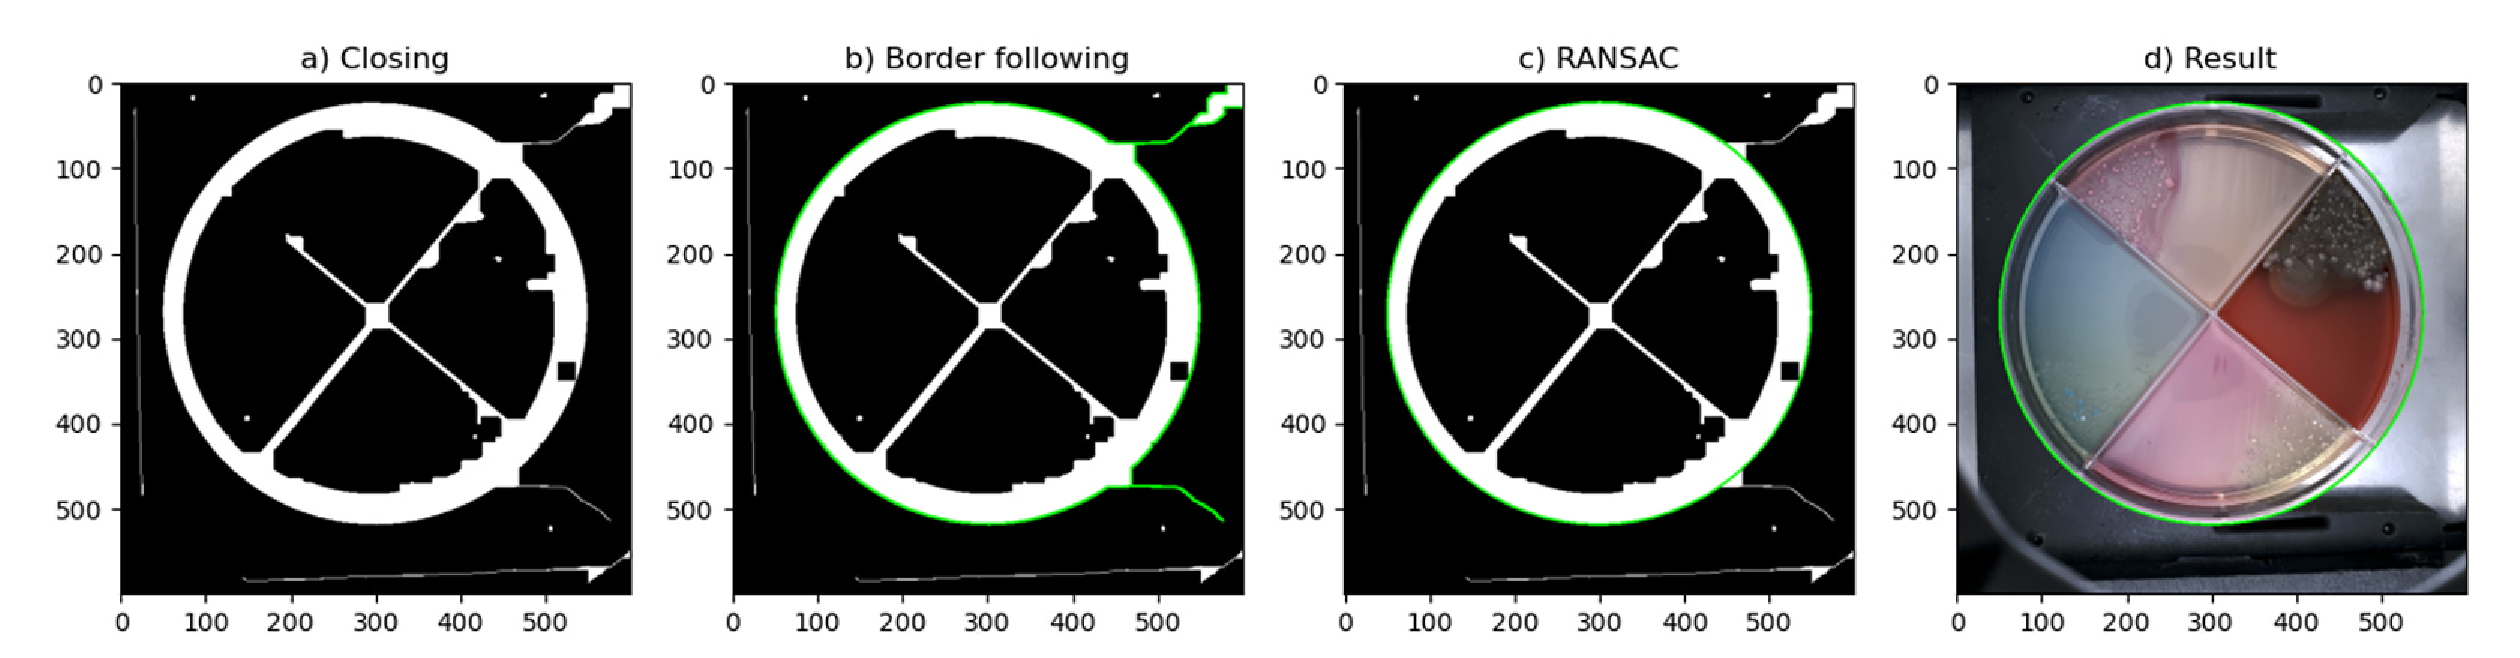
\includegraphics[width=1\linewidth]{figures/PDF/Ransac.pdf}\\
    \caption{a) Closing applied to fix broken canny edges. b) Border following of the outermost contour. c) RANSAC to fit an ellipse on the identified outer edge. d) The final contour of the agar plate identified.}
    \label{fig:result ransac}
\end{figure}

\noindent Lastly the ROI masking was made using the elliptical contour extracted from the RANSAC, which gave good results as seen in \textit{Figure \ref{fig:result mask})}
\begin{figure}[htbp]
    \centering
      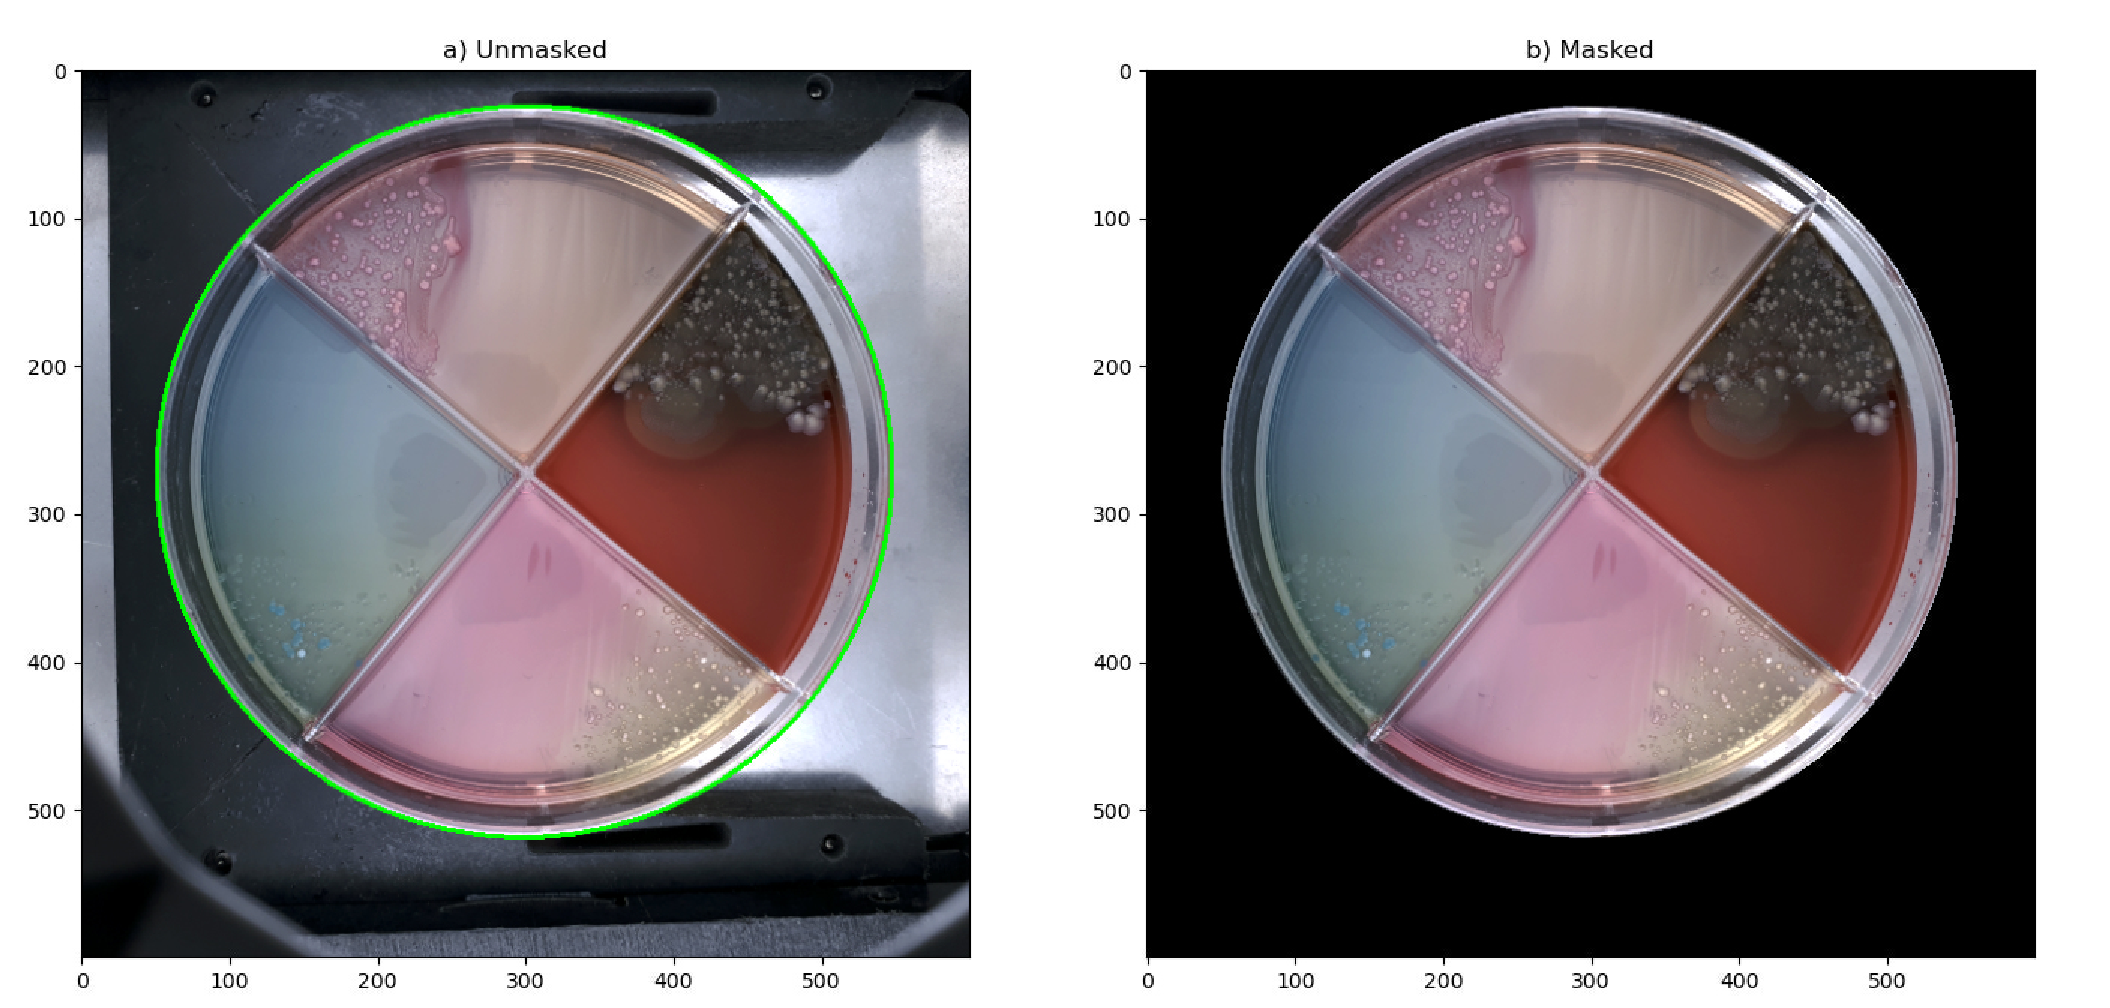
\includegraphics[width=.85\linewidth]{figures/PDF/Mask.pdf}\\
    \caption{a) Agar plate with detected outer contour. b) Pixels outside the outer contour masked . }
    \label{fig:result mask}
\end{figure}


\subsection{Identify compartment edges}
Canny, together with the additional Gaussian blur, proved to be an efficient method for identifying the compartment edges. The Gaussian blur sigma value was set to 1.2, a bit higher as opposed to the value in \textit{Section 5.1.1.} Canny still operated with the same lower and upper threshold values as before. As a consequence of bacteria clusters growing close to the compartment edges, some edges could not be identified properly. This resulted in some deviations, as seen in the second row of \text{Figure \ref{fig:result skeletonize} a)}.\\

\noindent Morphological Closing gave accurate results in merging any lines, as seen in \textit{Figure \ref{fig:result skeletonize} b)}. However, bacteria clusters close to the compartment edges did sometimes interfere with the edge, as in the second row of \textit{Figure \ref{fig:result skeletonize} b)}. \\

\noindent Lastly, the first row in \textit{Figure \ref{fig:result skeletonize} c)} shows that Skeletonization produced an accurate representation of the centermost edge in \textit{Figure \ref{fig:result skeletonize} b)}, while the input in the second row was affected by bacteria growing close to the edges. Fairly accurate final results of finding the compartment edges were still produced in both cases in \textit{Figure \ref{fig:result houghlines}}, due to the validation.

\begin{figure}[H]
    \centering
      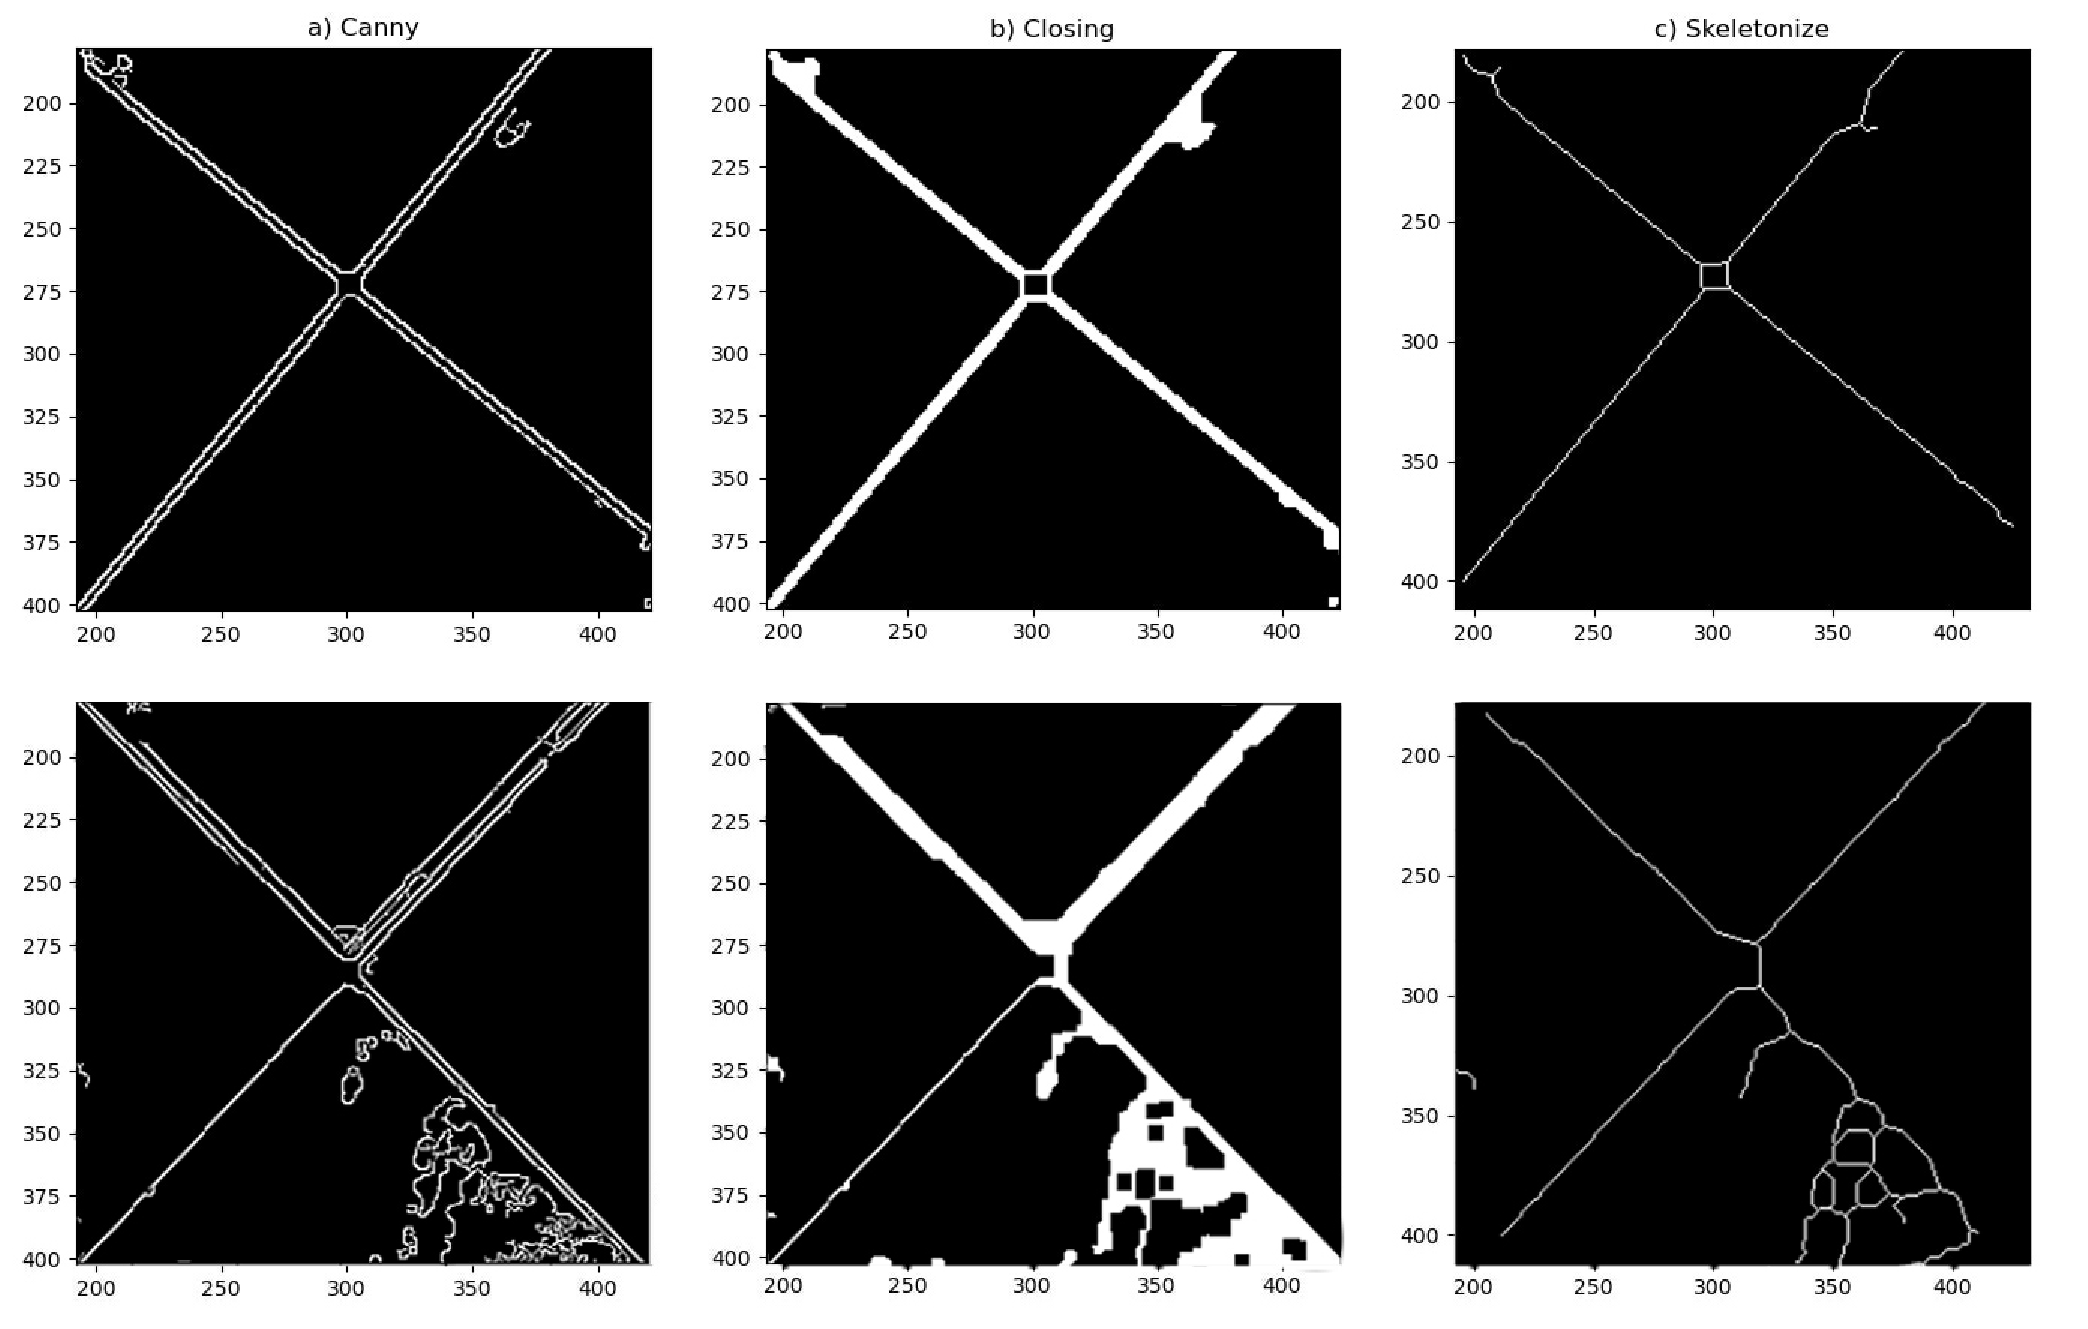
\includegraphics[width=1\linewidth]{figures/PDF/Skeletonize_double.pdf}\\
    \caption{a) Masked binary Canny image. b) Morphological Closing to form one thick line. c) Skeletonize of the thick line, giving a pixel-wide centerline.}
    \label{fig:result skeletonize}
\end{figure}


\begin{figure}[H]
    \centering
      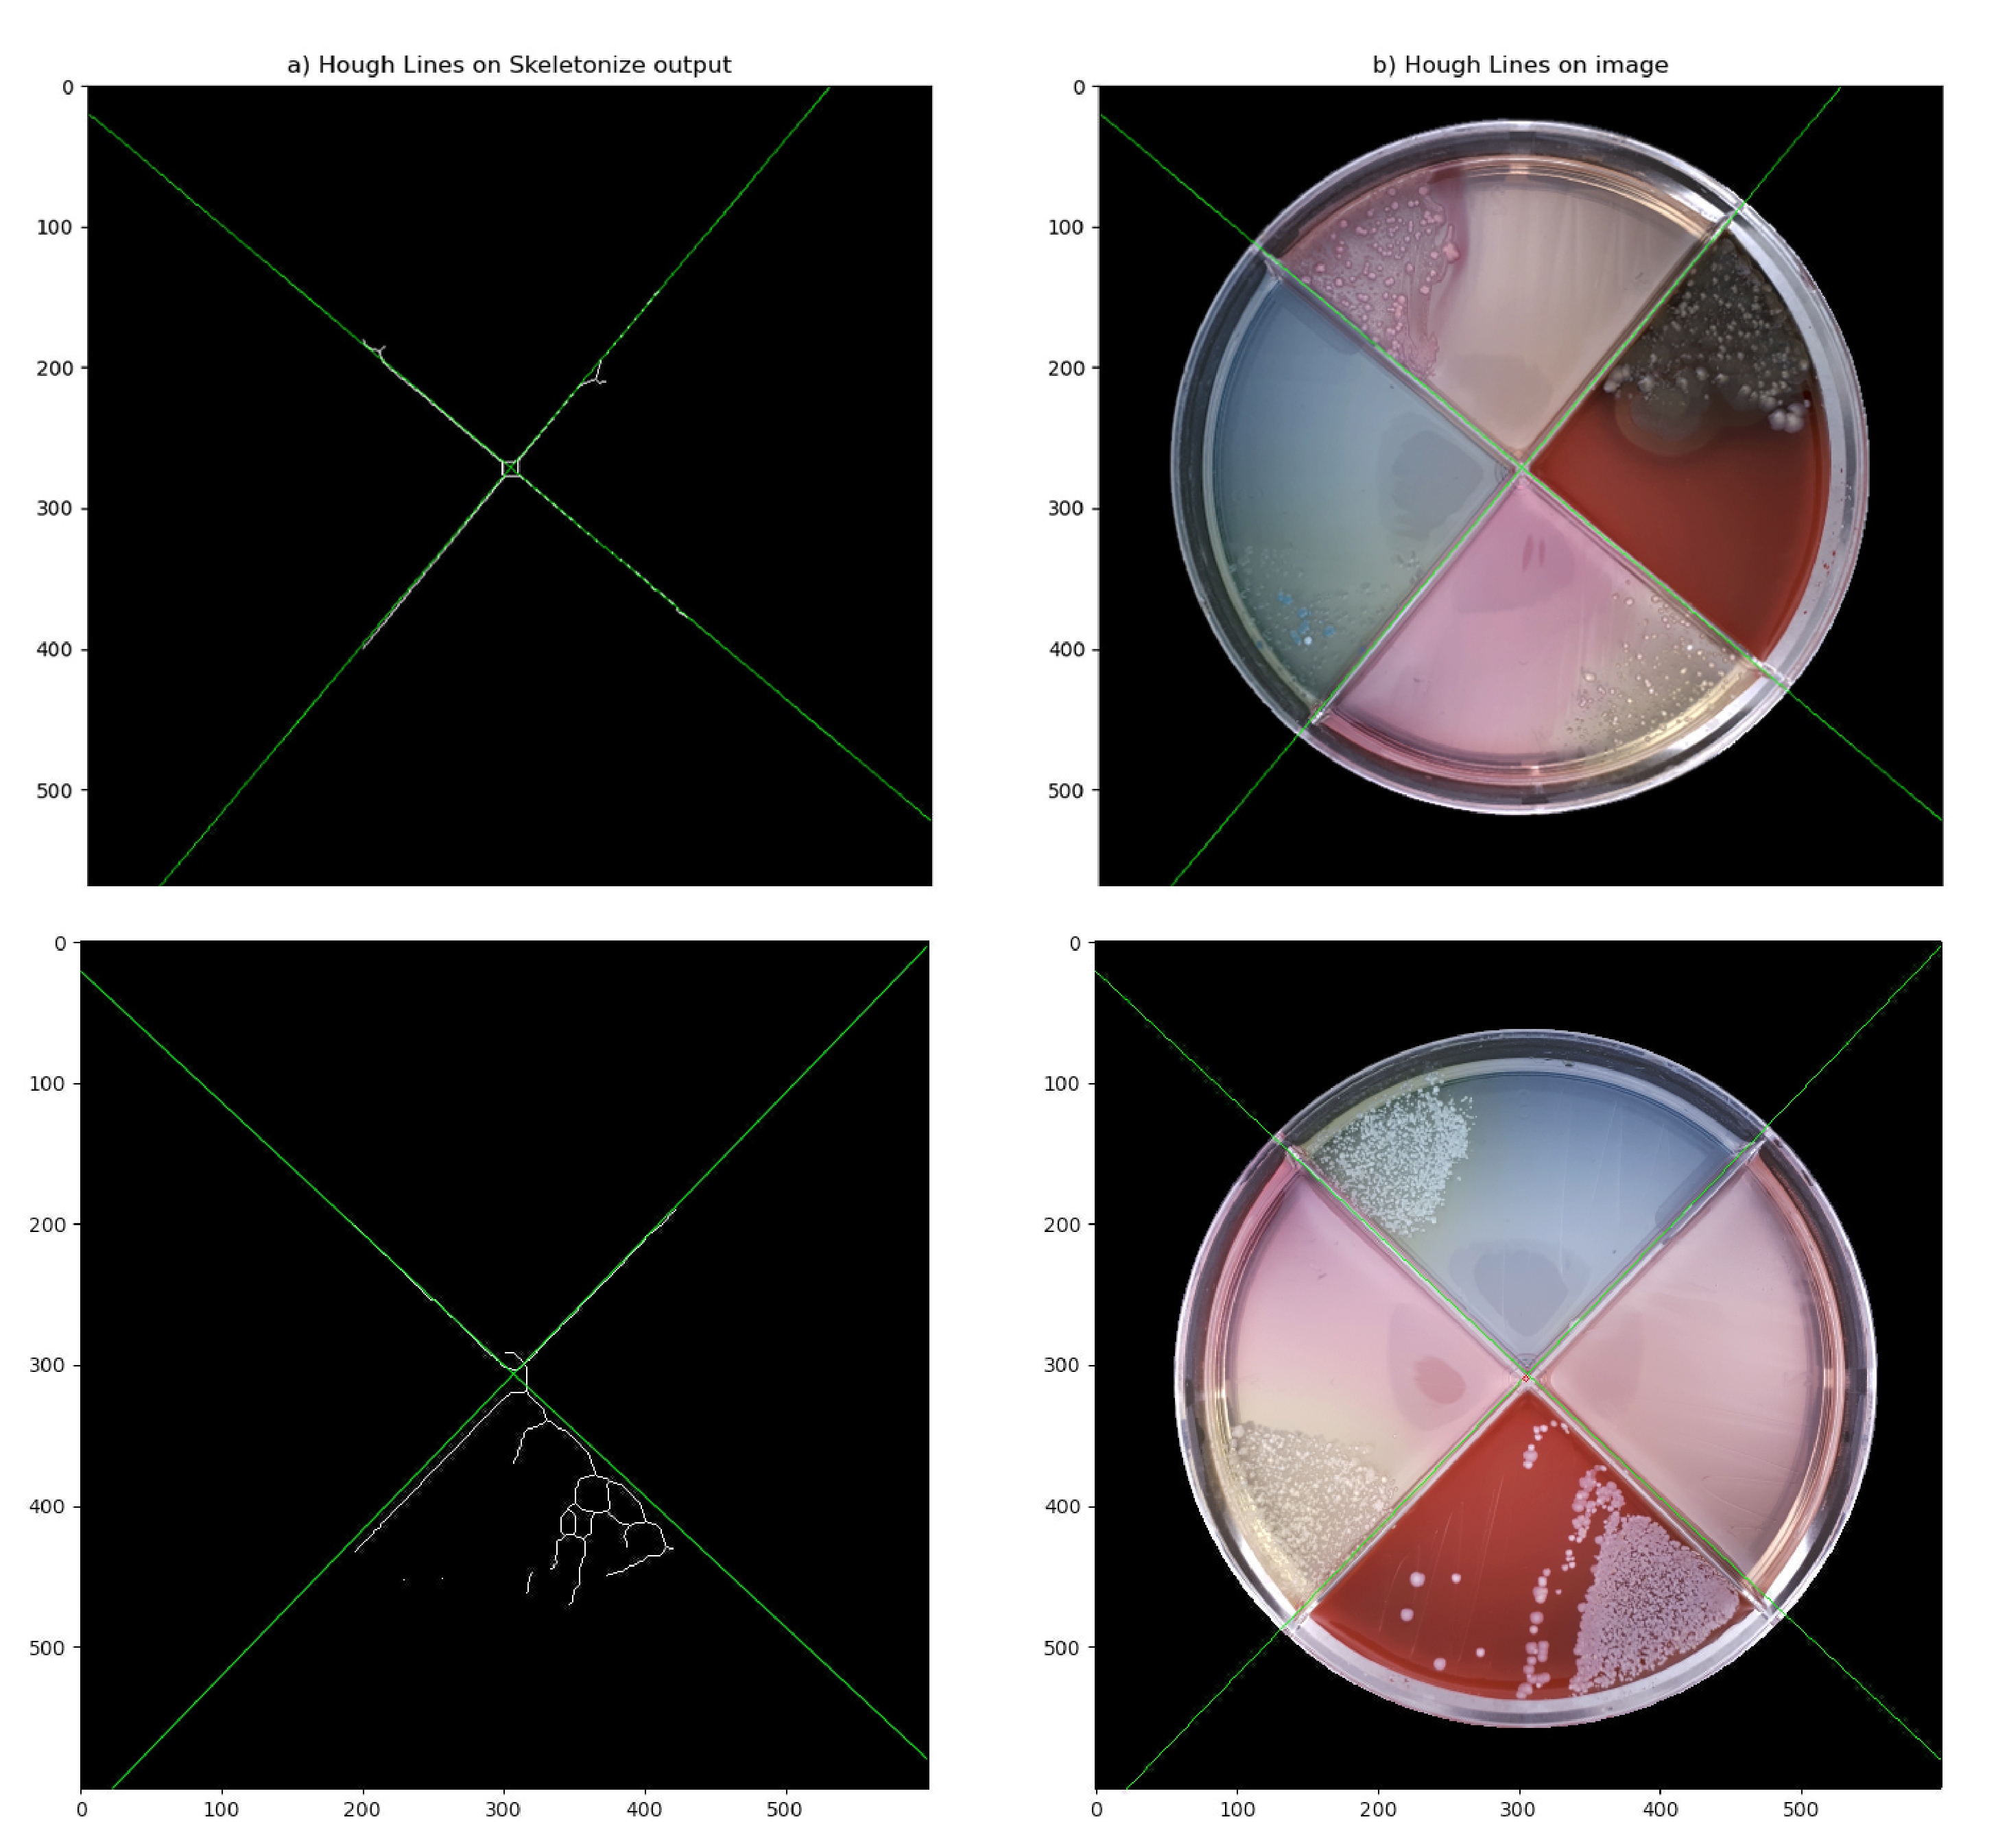
\includegraphics[width=.81\linewidth]{figures/PDF/Hough_lines_double.pdf}\\
    \caption{a) Lines found by Hough Lines over skeletonized output. b) The same lines are drawn over the input image.}
    \label{fig:result houghlines}
\end{figure}

\subsection{Identify agar plate orientation}
Changing the values within the HSV-space gave the most distinctive segmentation of any red pixels. HSV-values were selected to work for the whole dataset, which gave a lower threshold of [H = 0, S = 130, V = 0] and a upper threshold of [H = 179, S = 255, V = 255] to segment the red compartment (see \textit{Figure \ref{fig:result segmentation} b)}). Calculating the red RGB mean value of each line to identify the orientation proved to give consistent results. In many cases, it even worked without the segmentation, but the segmentation was still needed to give accurate results on the entire dataset. With the segmentation of the red compartment, the orientation could easily be identified, as seen in \textit{Figure \ref{fig:result segmentation} c)}. 

\begin{figure}[H]
    \centering
      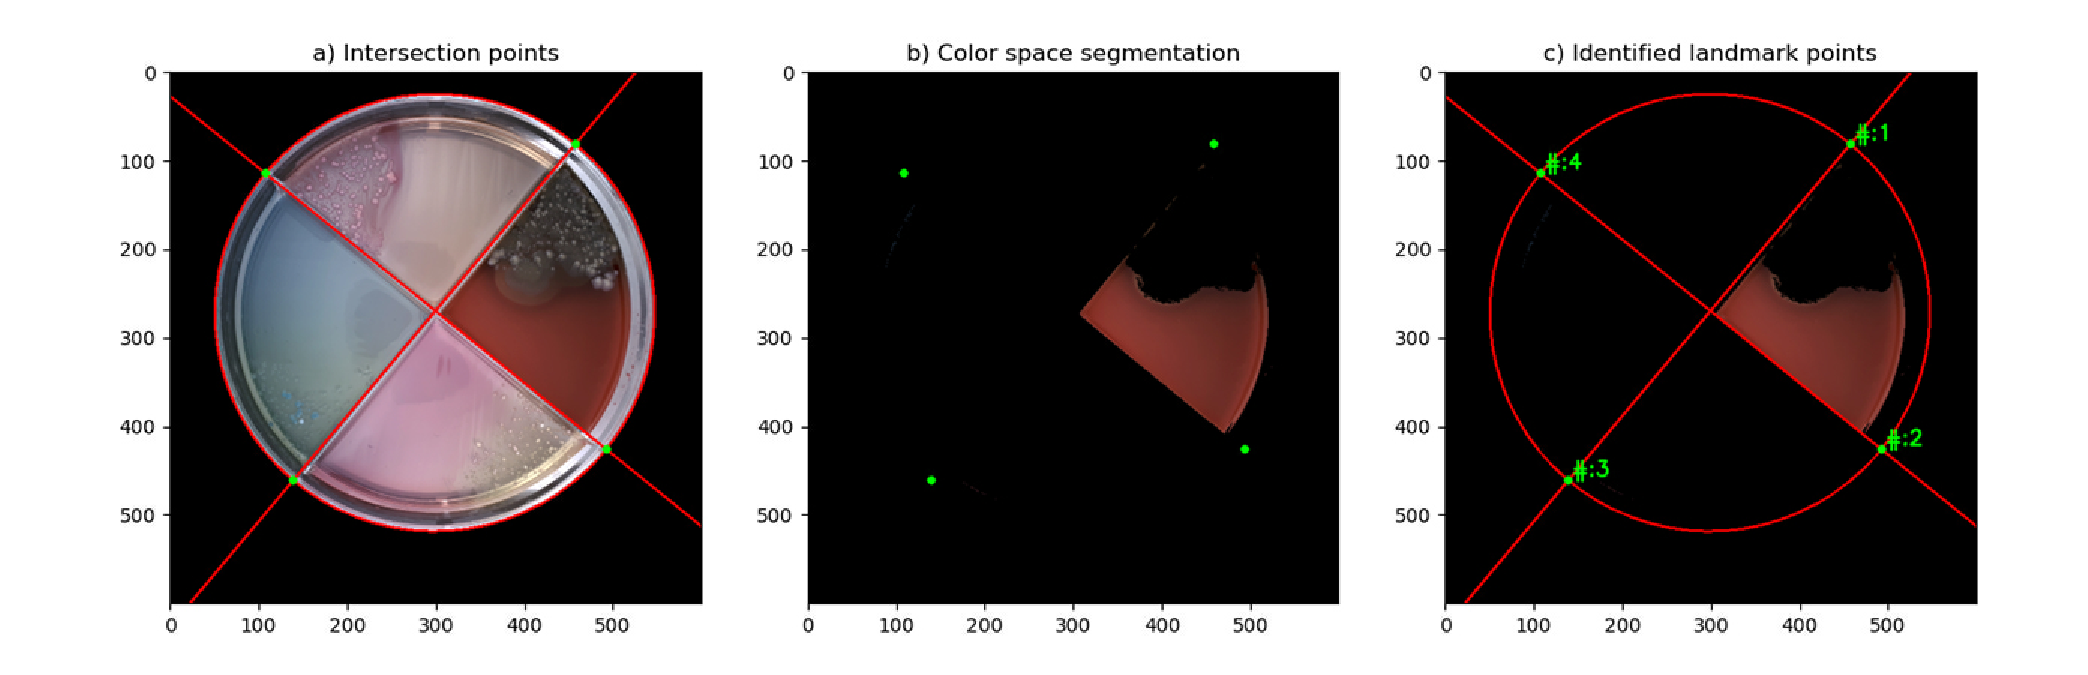
\includegraphics[width=.85\linewidth]{figures/PDF/Segmentation.pdf}\\
    \caption{a) Intersection points between the outer contour and the identified compartment edges. b) Segmented red compartment using color space segmentation. c) Sorted intersection points. }
    \label{fig:result segmentation}
\end{figure}

\subsection{Image registration}
As seen in \textit{Figure \ref{fig:result keys} a)}, key points were able to be matched to their corresponding reference points in \textit{Figure \ref{fig:result keys} b)}. The figure only shows a total of 37 key points for illustrational purposes. The final outputs in \textit{Figure \ref{fig:result final} d)} were processed with a total of 10 005 key points, divided into 2 500 key points per line, 5 000 for the ellipse, and 5 for the center and landmark points.\\  

\begin{figure}[H]
      \centering
      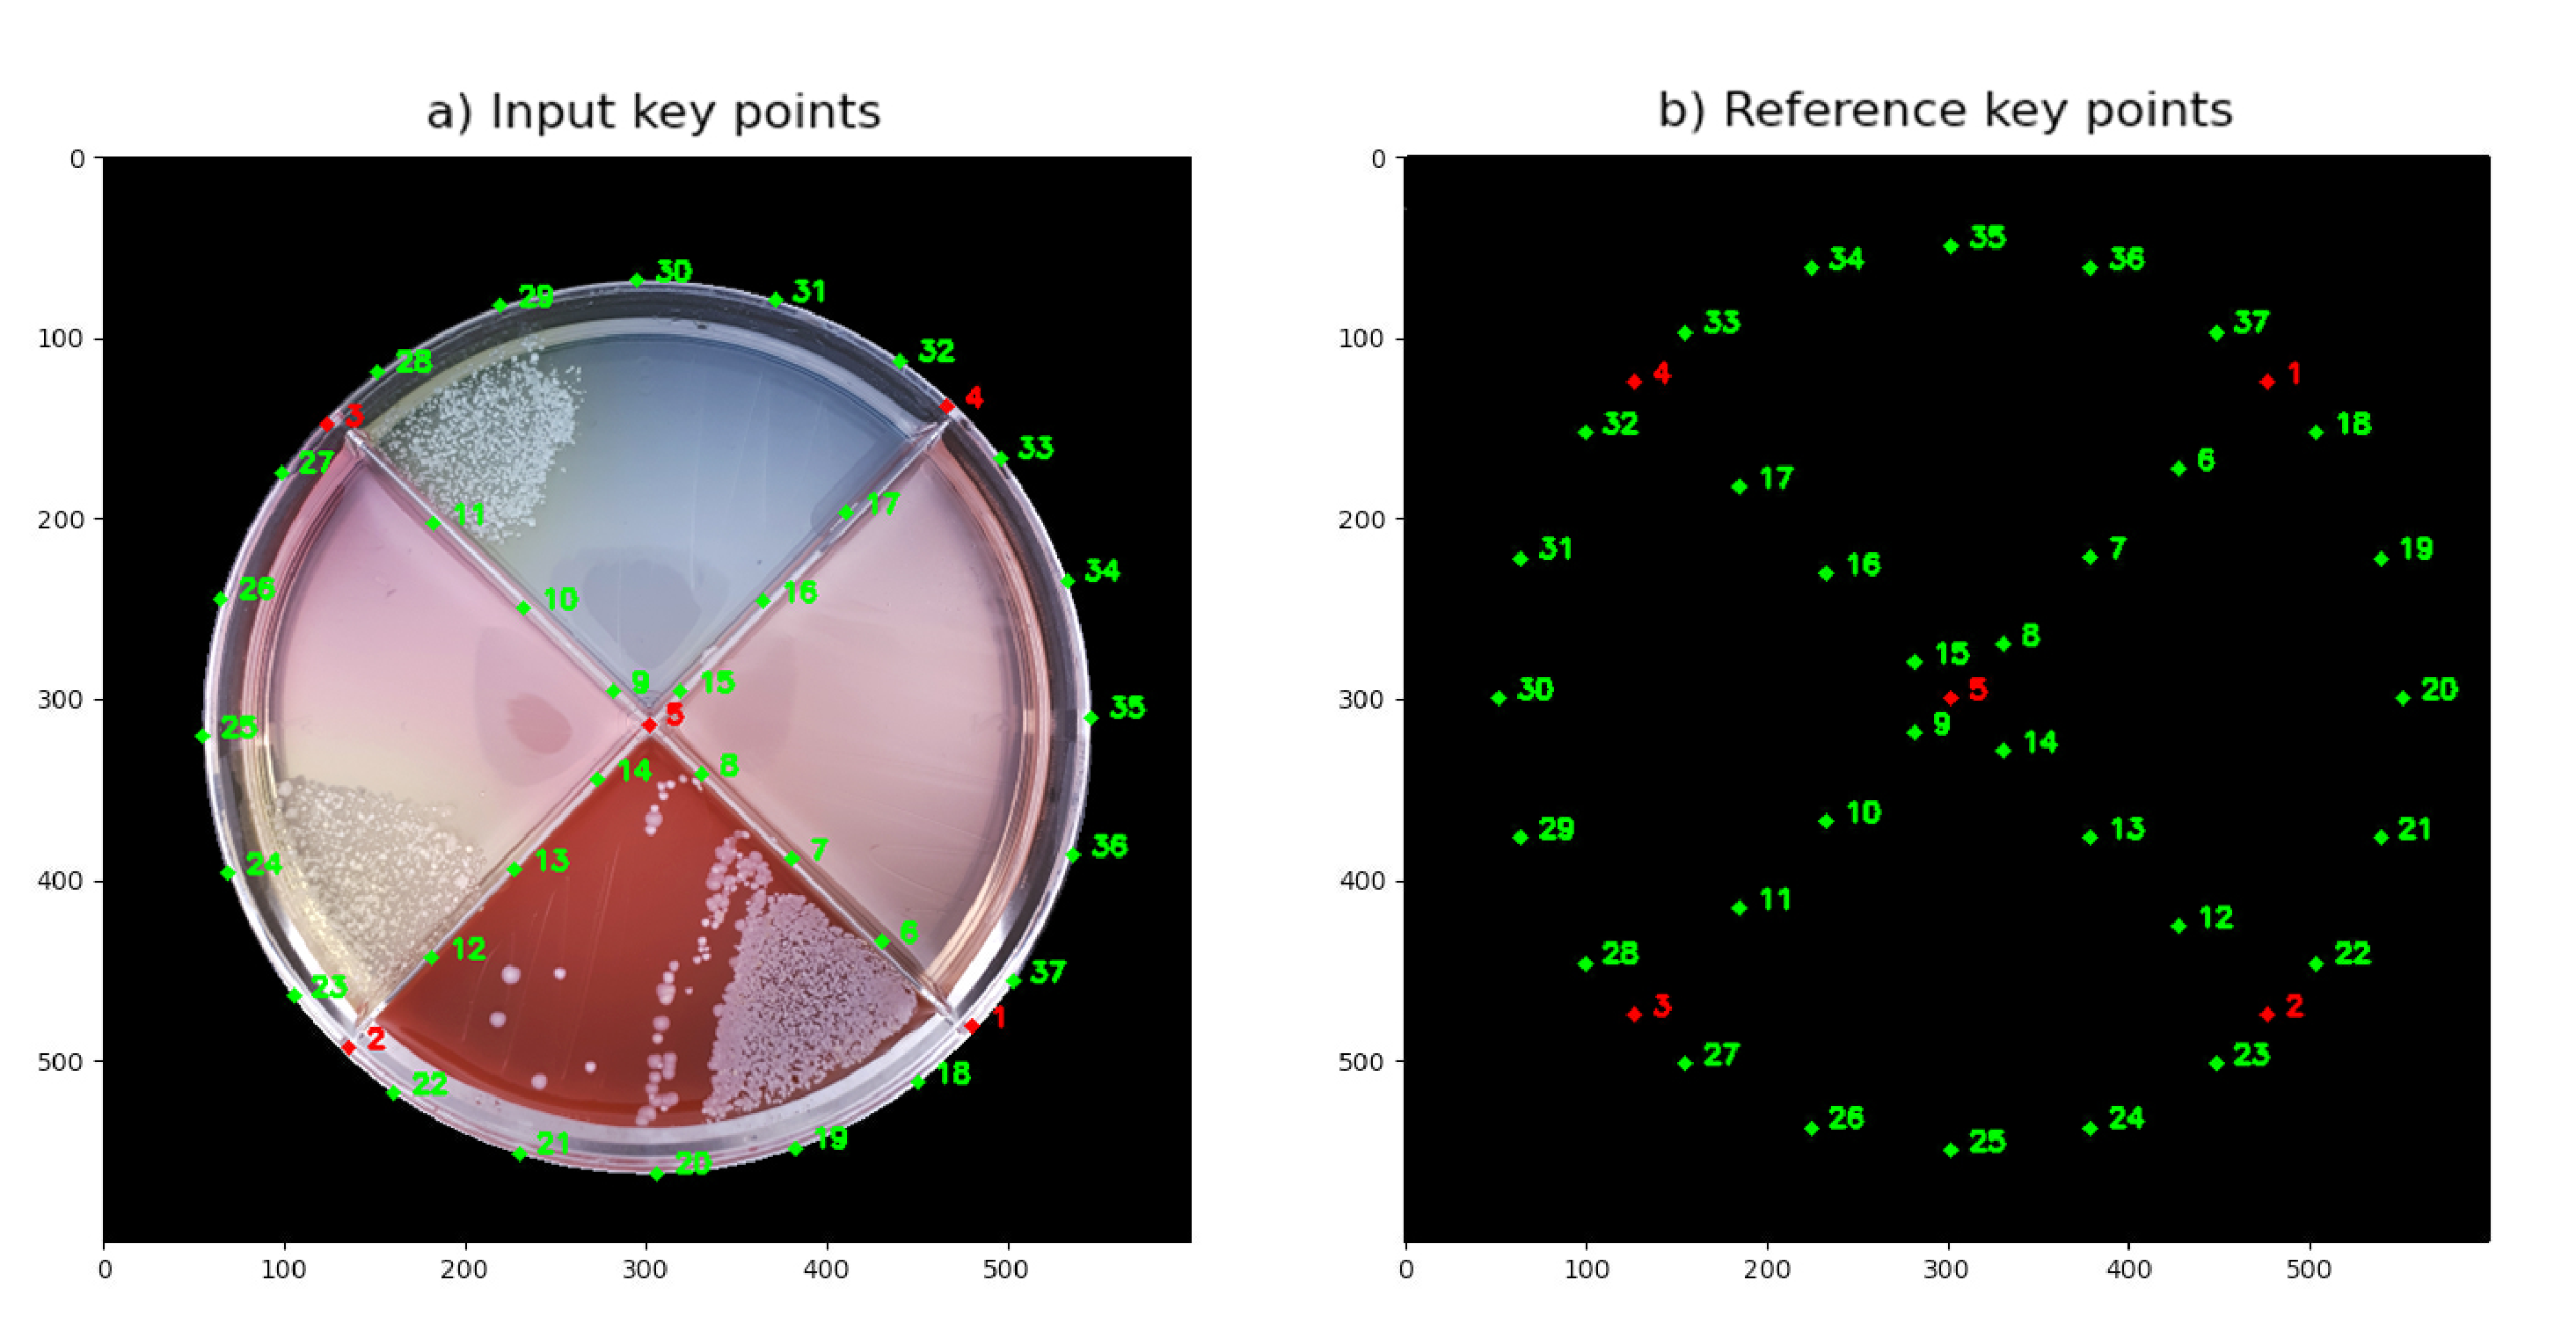
\includegraphics[width=0.9\linewidth]{figures/PDF/Image_reg.pdf}
    \caption{a) Identified key points for the input image. b) Reference key points.}
    \label{fig:result keys}
\end{figure}

\noindent Finally, \textit{Figure \ref{fig:result projection}} shows very promising results for any perspective distortion still occurring after the first full iteration. A second iteration provided a near-perfect, circular projection of the agar plate. 

\begin{figure}[H]
      \centering
      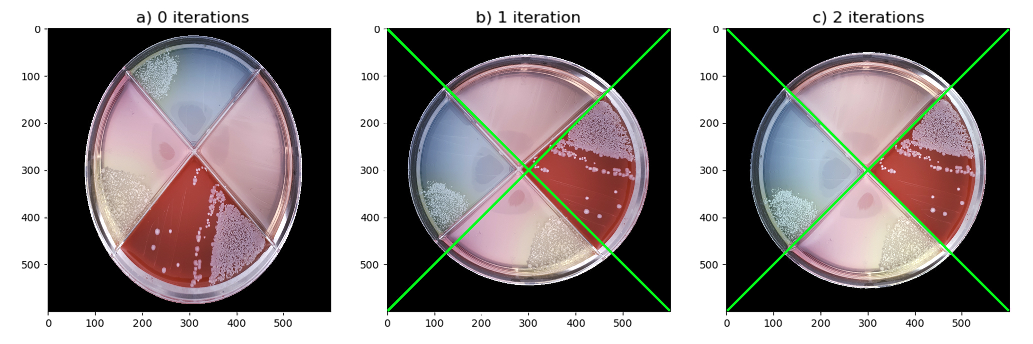
\includegraphics[width=1\linewidth]{figures/PDF/Projection.pdf}
    \caption{a) Image constructed with extreme perspective distortion before registration.  b) The result after one iteration. c) The result after two iterations.}
    \label{fig:result projection}
\end{figure}


\section{Evaluation}
Evaluating the final output proved that the outputs were valid considering a small margin of error. \textit{Figure \ref{fig:result evaluation} a)} shows a near-perfect transformation and rotation, while the remaining outputs show slight variations compared to the overlay template. However, the variations were minimal, and the red compartment was in all cases oriented to the right according to the green arrow throughout the data set. 
\begin{figure}[H]
      \centering
      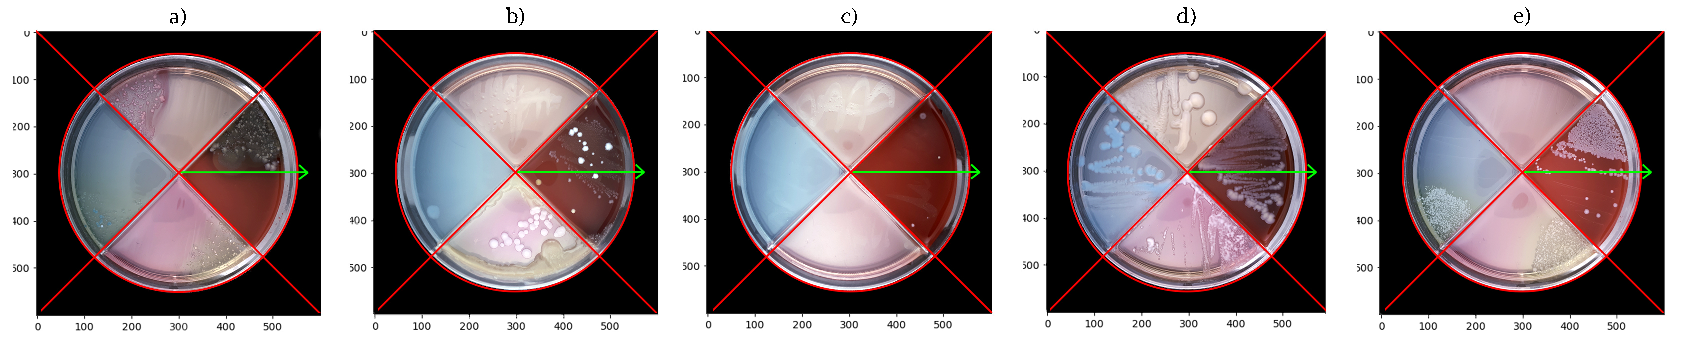
\includegraphics[width=1\linewidth]{figures/PDF/Evaluation_result.pdf}
    \caption{Validation of final output from \textit{Figure \ref{fig:result final} d)}}
    \label{fig:result evaluation}
\end{figure}





%%%%%%%%%%%%%%%%%%%%%%%%%%%%%%%%%%%%%%%%%%%%%%%%%%%%%%%%%%%%%%%%%%%%%%
%%% lorem.tex ends here

%%% Local Variables: 
%%% mode: latex
%%% TeX-master: "demothesis"
%%% End: 
